\documentclass[12pt,hidelinks]{article}
	\usepackage[explicit]{titlesec}
	\usepackage{titletoc}
	\usepackage{tocloft}
	\usepackage{charter}
	\usepackage[many]{tcolorbox}
	\usepackage{amsmath}
	\usepackage{graphicx}
	\usepackage{xcolor}
	\usepackage{tikz,lipsum,lmodern}
	\usetikzlibrary{calc}
	\usepackage[english]{babel}
	\usepackage{fancyhdr}
	\usepackage{mathrsfs}
	\usepackage{empheq}
	\usepackage{fourier}% change to lmodern if fourier is no available
	\usepackage{wrapfig}
	\usepackage{fancyref}
	\usepackage{hyperref}
	\usepackage{cleveref}
	\usepackage{listings}
	\usepackage{varwidth}
	\usepackage{longfbox}
	\usepackage{geometry}
	\usepackage{marginnote}
	\usepackage{amsmath}
	\tcbuselibrary{theorems}
	\tcbuselibrary{breakable, skins}
	\tcbuselibrary{listings, documentation}
	\geometry{
		a4paper,
		left=33mm,
		right=33mm,
		top=20mm}
% ========= Path to images ============
%   - Direct the computer on the path 
% 	  to the folder containg the images
% =====================================
\graphicspath{{./img/}}
% ============= Macros ================
\newcommand{\fillin}{\underline{\hspace{.75in}}{\;}}
\newcommand{\solution}{\textcolor{mordantred19}{Solution:}}
\setlength{\parindent}{0pt}
\setlength{\arrayrulewidth}{0.5mm}
\setlength{\tabcolsep}{18pt}
\addto{\captionsenglish}{\renewcommand*{\contentsname}{Table of Contents}}
\linespread{1.2}
% ======== Footers & Headers ==========
\cfoot{\thepage}
\chead{}\rhead{}\lhead{}
% =====================================
\renewcommand{\thesection}{\arabic{section}}
\newcommand\sectionnumfont{% font specification for the number
	\fontsize{380}{130}\color{myblueii}\selectfont}
\newcommand\sectionnamefont{% font specification for the name "PART"
	\normalfont\color{white}\scshape\small\bfseries }
% ============= Colors ================
% ----- Red -----
\definecolor{mordantred19}{rgb}{0.68, 0.05, 0.0}
% ----- Blue -----
\definecolor{st.patrick\'sblue}{rgb}{0.14, 0.16, 0.48}
\definecolor{teal}{rgb}{0.0, 0.5, 0.5}
\definecolor{beaublue}{rgb}{0.74, 0.83, 0.9}
\definecolor{mybluei}{RGB}{0,173,239}
\definecolor{myblueii}{RGB}{63,200,244}
\definecolor{myblueiii}{RGB}{199,234,253}
% ---- Yellow ----
\definecolor{blond}{rgb}{0.98, 0.94, 0.75}
\definecolor{cream}{rgb}{1.0, 0.99, 0.82}
% ----- Green ------
\definecolor{emerald}{rgb}{0.31, 0.78, 0.47}
\definecolor{darkspringgreen}{rgb}{0.09, 0.45, 0.27}
% ---- White -----
\definecolor{ghostwhite}{rgb}{0.97, 0.97, 1.0}
\definecolor{splashedwhite}{rgb}{1.0, 0.99, 1.0}
% ---- Grey -----
\definecolor{whitesmoke}{rgb}{0.96, 0.96, 0.96}
\definecolor{lightgray}{rgb}{0.92, 0.92, 0.92}
\definecolor{floralwhite}{rgb}{1.0, 0.98, 0.94}
% ========= Part Format ==========
\titleformat{\section}
{\normalfont\huge\filleft}
{}
{20pt}
{\begin{tikzpicture}[remember picture,overlay]
	\fill[myblueiii] 
	(current page.north west) rectangle ([yshift=-13cm]current page.north east);   
\node[
	fill=mybluei,
	text width=2\paperwidth,
	rounded corners=6cm,
	text depth=18cm,
	anchor=center,
	inner sep=0pt] at (current page.north east) (parttop)
	{\thepart};%
\node[
	anchor=south east,
	inner sep=0pt,
	outer sep=0pt] (partnum) at ([xshift=-20pt]parttop.south) 
	{\sectionnumfont\thesection};
\node[
	anchor=south,
	inner sep=0pt] (partname) at ([yshift=2pt]partnum.south)   
	{\sectionnamefont SECTION};
\node[
	anchor=north east,
	align=right,
	inner xsep=0pt] at ([yshift=-0.5cm]partname.east|-partnum.south) 
	{\parbox{.7\textwidth}{\raggedleft#1}};
\end{tikzpicture}%
}
% ========= Hyper Ref ===========
\hypersetup{
	colorlinks,
	linkcolor={red!50!black},
	citecolor={blue!50!black},
	urlcolor={blue!80!black}
}
% ========= Example Boxes =============
\tcbset{
	defstyle/.style={
		fonttitle=\bfseries\upshape, 
		fontupper=\slshape,
		arc=0mm, 
		beamer,
		colback=blue!5!white,
		colframe=blue!75!black},
	theostyle/.style={
		fonttitle=\bfseries\upshape, 
		fontupper=\slshape,
		colback=red!10!white,
		colframe=red!75!black},
	visualstyle/.style={
		height=6.5cm,
		breakable,
		enhanced,
		leftrule=0pt,
		rightrule=0pt,
		bottomrule=0pt,
		outer arc=0pt,
		arc=0pt,
		colframe=mordantred19,
		colback=lightgray,
		attach boxed title to top left,
		boxed title style={
			colback=mordantred19,
			outer arc=0pt,
			arc=0pt,
			top=3pt,
			bottom=3pt,
		},
		fonttitle=\sffamily,},
	discussionstyle/.style={
		height=6.5cm,
		breakable,
		enhanced,
		rightrule=0pt,
		toprule=0pt,
		outer arc=0pt,
		arc=0pt,
		colframe=mordantred19,
		colback=lightgray,
		attach boxed title to top left,
		boxed title style={
			colback=mordantred19,
			outer arc=0pt,
			arc=0pt,
			top=3pt,
			bottom=3pt,
		},
		fonttitle=\sffamily},
	mystyle/.style={
		height=6.5cm,
		breakable,
		enhanced,
		rightrule=0pt,
		leftrule=0pt,
		bottomrule=0pt,
		outer arc=0pt,
		arc=0pt,
		colframe=mordantred19,
		colback=lightgray,
		attach boxed title to top left,
		boxed title style={
			colback=mordantred19,
			outer arc=0pt,
			arc=0pt,
			top=3pt,
			bottom=3pt,
		},
		fonttitle=\sffamily},
	aastyle/.style={
			height=3.5cm,
			enhanced,
			colframe=teal,
			colback=lightgray,
			colbacktitle=floralwhite,
			fonttitle=\bfseries,
			coltitle=black,
		attach boxed title to top center={
	  		yshift=-0.25mm-\tcboxedtitleheight/2,
	   		yshifttext=2mm-\tcboxedtitleheight/2}, 
		boxed title style={boxrule=0.5mm,
			frame code={ \path[tcb fill frame] ([xshift=-4mm]frame.west)
				-- (frame.north west) -- (frame.north east) -- ([xshift=4mm]frame.east)
				-- (frame.south east) -- (frame.south west) -- cycle; },
			interior code={ 
				\path[tcb fill interior] ([xshift=-2mm]interior.west)
				-- (interior.north west) -- (interior.north east)
				-- ([xshift=2mm]interior.east) -- (interior.south east) -- (interior.south west)
				-- cycle;} }
				},
	examstyle/.style={
		height=9.5cm,
		breakable,
		enhanced,
		rightrule=0pt,
		leftrule=0pt,
		bottomrule=0pt,
		outer arc=0pt,
		arc=0pt,
		colframe=mordantred19,
		colback=lightgray,
		attach boxed title to top left,
		boxed title style={
			colback=mordantred19,
			outer arc=0pt,
			arc=0pt,
			top=3pt,
			bottom=3pt,
		},
		fonttitle=\sffamily},
	doc head command={
		interior style={
			fill,
			left color=yellow!20!white, 
			right color=white}},
	doc head environment={
		boxsep=4pt,
		arc=2pt,
		colback=yellow!30!white,
		},
	doclang/environment content=text
}
% ============= Boxes ================
\newtcolorbox[auto counter,number within=section]{example}[1][]{
	mystyle,
	title=Example~\thetcbcounter,
	overlay unbroken and first={
		\path
		let
		\p1=(title.north east),
		\p2=(frame.north east)
		in
		node[anchor=
			west,
			font=\sffamily,
			color=st.patrick\'sblue,
			text width=\x2-\x1] 
		at (title.east) {#1};
	}
}
\newtcolorbox[auto counter,number within=section]{longexample}[1][]{
	examstyle,
	title=Example~\thetcbcounter,
	overlay unbroken and first={
		\path
		let
		\p1=(title.north east),
		\p2=(frame.north east)
		in
		node[anchor=
		west,
		font=\sffamily,
		color=st.patrick\'sblue,
		text width=\x2-\x1] 
		at (title.east) {#1};
	}
}
\newtcolorbox[auto counter,number within=section]{example2}[1][]{
	aastyle,
	title=Example~\thetcbcounter,{}
}
\newtcolorbox[auto counter,number within=section]{discussion}[1][]{
	discussionstyle,
	title=Discussion~\thetcbcounter,
	overlay unbroken and first={
		\path
		let
		\p1=(title.north east),
		\p2=(frame.north east)
		in
		node[anchor=
		west,
		font=\sffamily,
		color=st.patrick\'sblue,
		text width=\x2-\x1] 
		at (title.east) {#1};
	}
}
\newtcolorbox[auto counter,number within=section]{visualization}[1][]{
	visualstyle,
	title=Visualization~\thetcbcounter,
	overlay unbroken and first={
		\path
		let
		\p1=(title.north east),
		\p2=(frame.north east)
		in
		node[anchor=
		west,
		font=\sffamily,
		color=st.patrick\'sblue,
		text width=\x2-\x1] 
		at (title.east) {#1};
	}
}
% --------- Theorems ---------
\newtcbtheorem[number within=subsection,crefname={definition}{definitions}]%
	{Definition}{Definition}{defstyle}{def}%
\newtcbtheorem[use counter from=Definition,crefname={theorem}{theorems}]%
	{Theorem}{Theorem}{theostyle}{theo}
	%
\newtcbtheorem[use counter from=Definition]{theo}{Theorem}%
{
	theorem style=plain,
	enhanced,
	colframe=blue!50!black,
	colback=yellow!20!white,
	coltitle=red!50!black,
	fonttitle=\upshape\bfseries,
	fontupper=\itshape,
	drop fuzzy shadow=blue!50!black!50!white,
	boxrule=0.4pt}{theo}
\newtcbtheorem[use counter from=Definition]{DashedDefinition}{Definition}%
 {
 	enhanced,
 	frame empty,
 	interior empty,
 	colframe=darkspringgreen!50!white,
	coltitle=darkspringgreen!50!black,
	fonttitle=\bfseries,
	colbacktitle=darkspringgreen!15!white,
	borderline={0.5mm}{0mm}{darkspringgreen!15!white},
	borderline={0.5mm}{0mm}{darkspringgreen!50!white,dashed},
	attach boxed title to top center={yshift=-2mm},
	boxed title style={boxrule=0.4pt},
	varwidth boxed title}{theo}
%%%%%%%%%%%%%%%%%%%%%%%%%%%%%%%%%%%%%%%%
\newtcblisting[auto counter,number within=section]{disexam}{
	skin=bicolor,
	colback=white!30!beaublue,
	colbacklower=white,
	colframe=black,
	before skip=\medskipamount,
	after skip=\medskipamount,
	fontlower=\footnotesize,
	listing options={style=tcblatex,texcsstyle=*\color{red!70!black}},}
%%%%%%%%%%%%%%%%%%%%%%%%%%%%%%%%%%%%%%%

\begin{document}
\begin{titlepage}
	\centering % Center everything on the title page
	\scshape % Use small caps for all text on the title page
	\vspace*{1.5\baselineskip} % White space at the top of the page
% ===================
%	Title Section 	
% ===================

	\rule{13cm}{1.6pt}\vspace*{-\baselineskip}\vspace*{2pt} % Thick horizontal rule
	\rule{13cm}{0.4pt} % Thin horizontal rule
	
		\vspace{0.75\baselineskip} % Whitespace above the title
% ========== Title ===============	
	{	\Huge InsuLink\\ 
			\vspace{4mm}
		Documentation \\	}
% ======================================
		\vspace{0.75\baselineskip} % Whitespace below the title
	\rule{13cm}{0.4pt}\vspace*{-\baselineskip}\vspace{3.2pt} % Thin horizontal rule
	\rule{13cm}{1.6pt} % Thick horizontal rule
	
		\vspace{1.75\baselineskip} % Whitespace after the title block
% =================
%	Information	
% =================
	{\large Produced by: Nicola Dean and Marco Fasanella \\
		\vspace*{1.2\baselineskip}
	CP: 10674826,10617541} \\
	\vfill
	\includegraphics[width=\textwidth]{logo}

\end{titlepage}
%%%%%%%%%%%%%%%%%%%%%%%%%%%%%%%%%%%%%%%%%%%%%%%%%%%%%%%%%%%
\tableofcontents
\vfill
\newpage
\newgeometry{
	left=29mm, 
	right=29mm, 
	top=20mm, 
	bottom=15mm}
%%%%%%%%%%%%%%%%%%%%%%%%%%%%%%%%%%%%%%%%%%%%%%%%%%%%%%%%%%%
\section{Idea}
\vspace{10.5cm}
When Type 1 Diabetes\cite{Type 1 Diabetes} is diagnosed, a patient starts a new life with different eyes. From now on, the conception of food is completely different
from the normal one, and the patient has to assimilate the big change and learn how to handle the disease. 
One of the most difficult but at the same time important things that the patient must learn, is the \textbf{\emph{carbohydrates count}} and subsequently the correct insulin dose for a bolus \cite{Bolus}.
InsuLink has been designed with the main purpose of giving an hand to Type 1 Diabetes patient with the calculation of the correct \textbf{\emph{insulin doses}} and  storing Glycemia values.
	\subsection{Main Goal}
    InsuLink main goal is to give a first support to the patient but only if combined with the doctor supervision. It is important to underline
	that this application is only defined by an algorithm, and in this kind of diseases \textbf{\emph{each patient 
	needs ad hoc treatments}}.

		\begin{docCommand}{usepackage}{}
			or
			\begin{verbatim}
				\usepackage{package}
			\end{verbatim}
		\end{docCommand}
	\vspace{-1.5mm}
\newpage
%%%%%%%%%%%%%%%%%%%%%%%%%%%%%%%%%%%%%%%%%%%%%%%%%%%%%%%%%%%
\section{Functionalities}
\vspace{10.5cm}
Insulink offers some useful tools to keep track of the daily routine of a patient. 
	\subsection{Food Scan}	
	It is possible to to scan a given Food BarCode and be redirectd to the FoodDetails page with all necessary data.
	\subsection{Glycemia}
    Keep track of your daily Glycemia with intuitive charts and easly with the glycemia insertion tool.

	\subsection{Insulin Calculator}
    An algorithm (inside Insulin Calculator class) will retrieve last Glycemia, total amount of carbohydrates, sport activity and all essential data
	to calculate the optimal insulin dose for the given meal. A more detailed explaintation can be fount in the Insulin Calculator Section.

	\subsection{Calendar}
	The user can see a well detailed sight of all previous data, just choosing a date from the InsuLink calendar, that will retrieve all the informations
	about that day from the database.
	
\newpage
%%%%%%%%%%%%%%%%%%%%%%%%%%%%%%%%%%%%%%%%%%%%%%%%%%%%%%%%%%%
\section{Screens and Navigation}
\vspace{10.5cm}
The following provides a screenshot of the pages with a brief description of their use.
	\subsection{Screens}
	\paragraph{Home}
    Home menu offers shortcuts to the main functionalities and a quick sight of the today glycemia with its intuitive charts.
	\begin{center}

	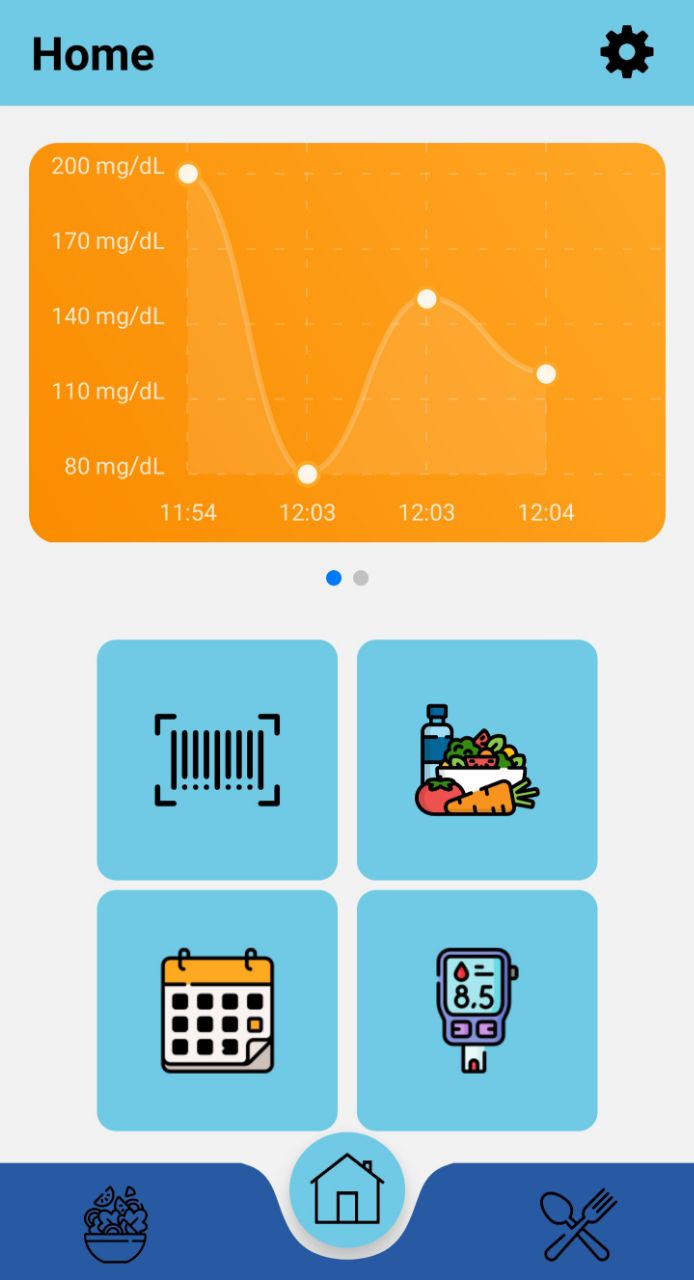
\includegraphics[scale=0.2]{screenshot3}
\end{center}

	\paragraph{Search}
    Search food or recipe for nutritional details or to add it in meal diary. User can easly modify the unit measure and quantity of food.
	\begin{center}

		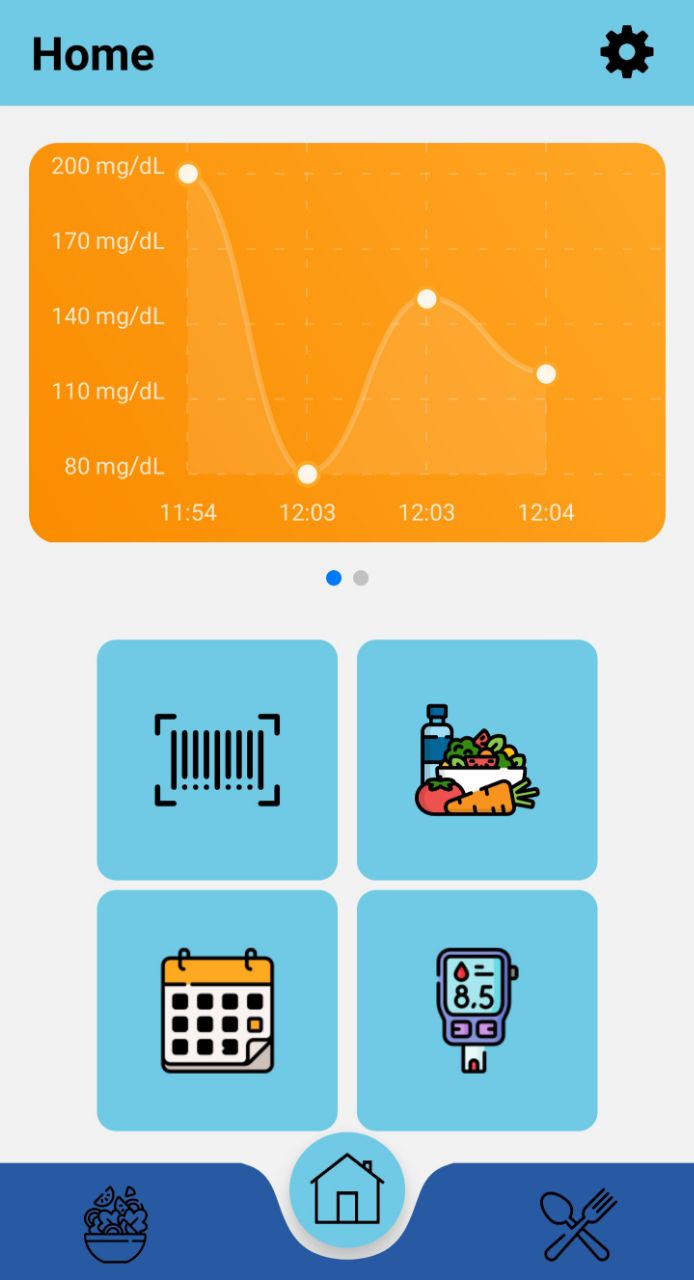
\includegraphics[scale=0.2]{screenshot3}
	\end{center}

	\paragraph{Glycemia PopUp}
    Add glycemia quickly just using the menu shortcut or during the insulin caluclation procedure. The value 
	will automatically stored in Firebase.
	\begin{center}

		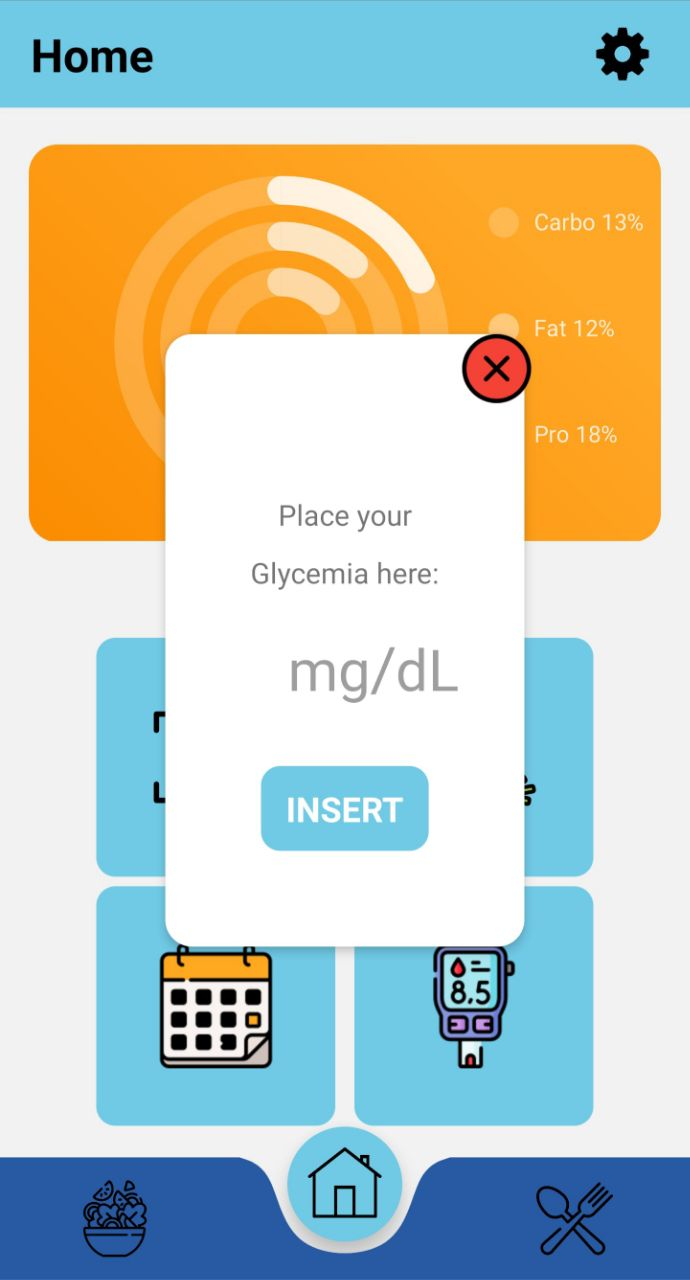
\includegraphics[scale=0.2]{screenshot1}
	\end{center}


	\paragraph{Meal Diary}
    Meal Diary can be used for both calulating daily total macro nutrients and insulin dose of each meal. 
	\begin{center}

		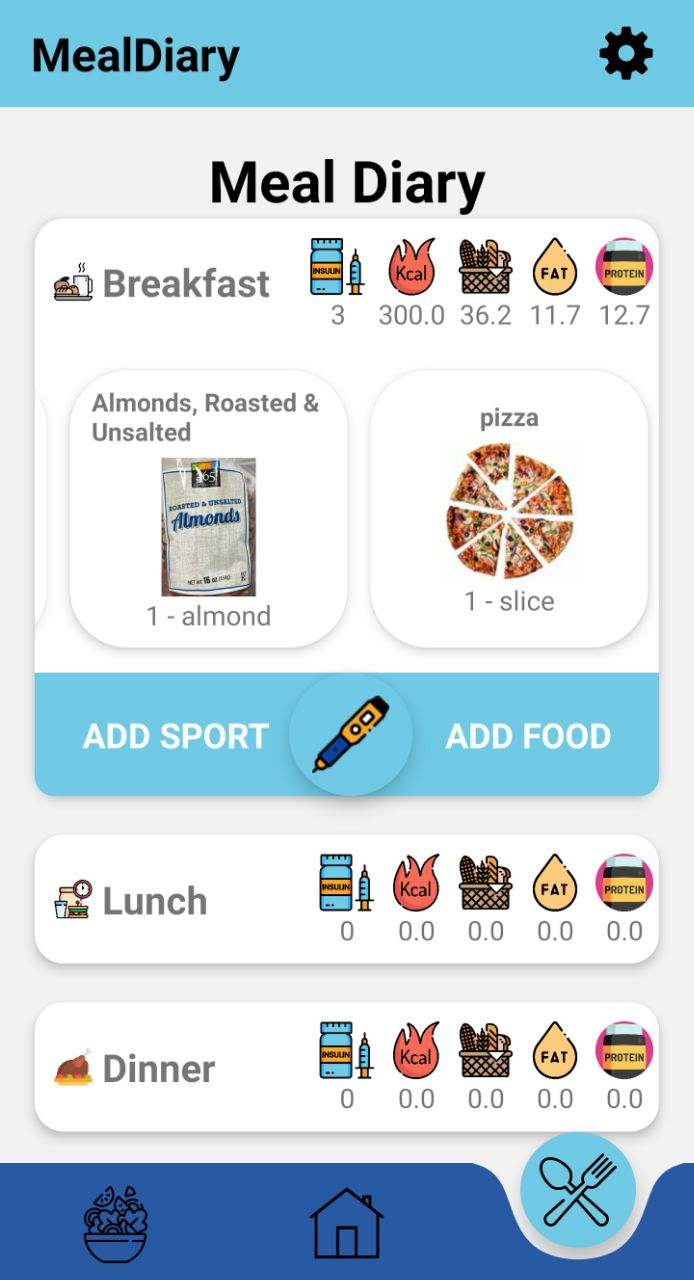
\includegraphics[scale=0.2]{screenshot5}
	\end{center}

	\paragraph{Calendar}
	In calendar it will be possible to retrieve historical data by clicking on a date. 
	\begin{center}

	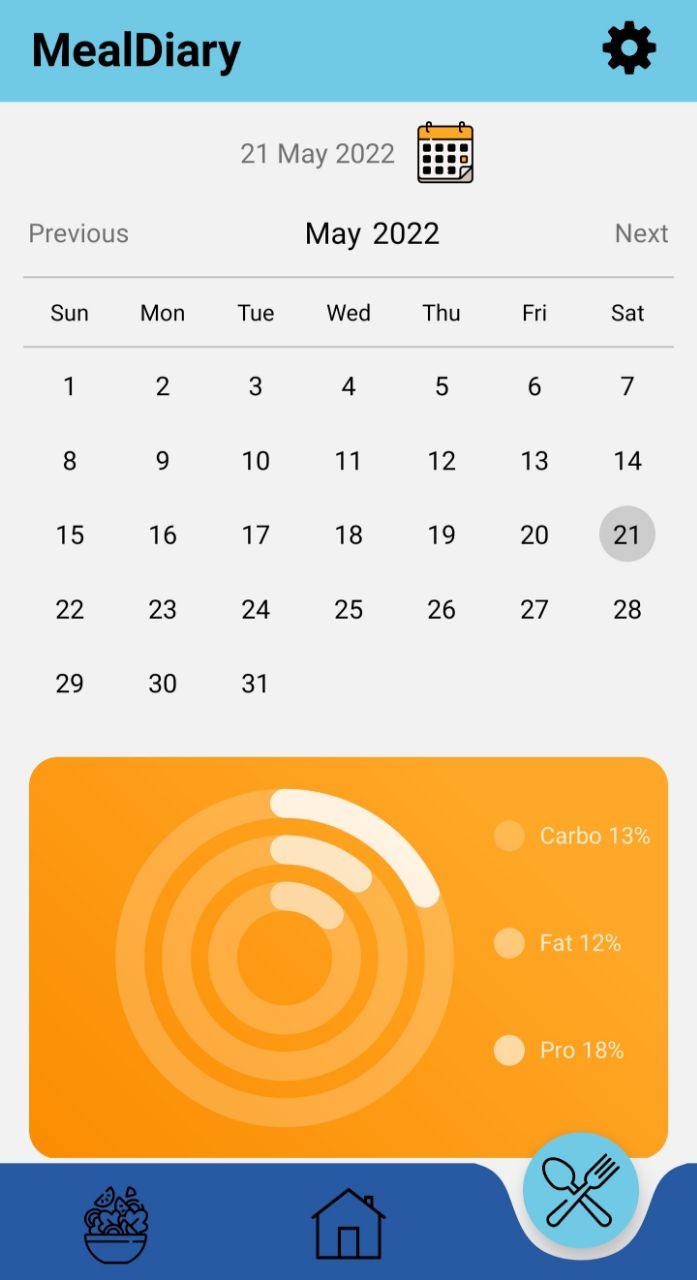
\includegraphics[scale=0.2]{screenshot4}
\end{center}
\newpage
\subsection{Navigation}

\paragraph{Registration}

\begin{center}
	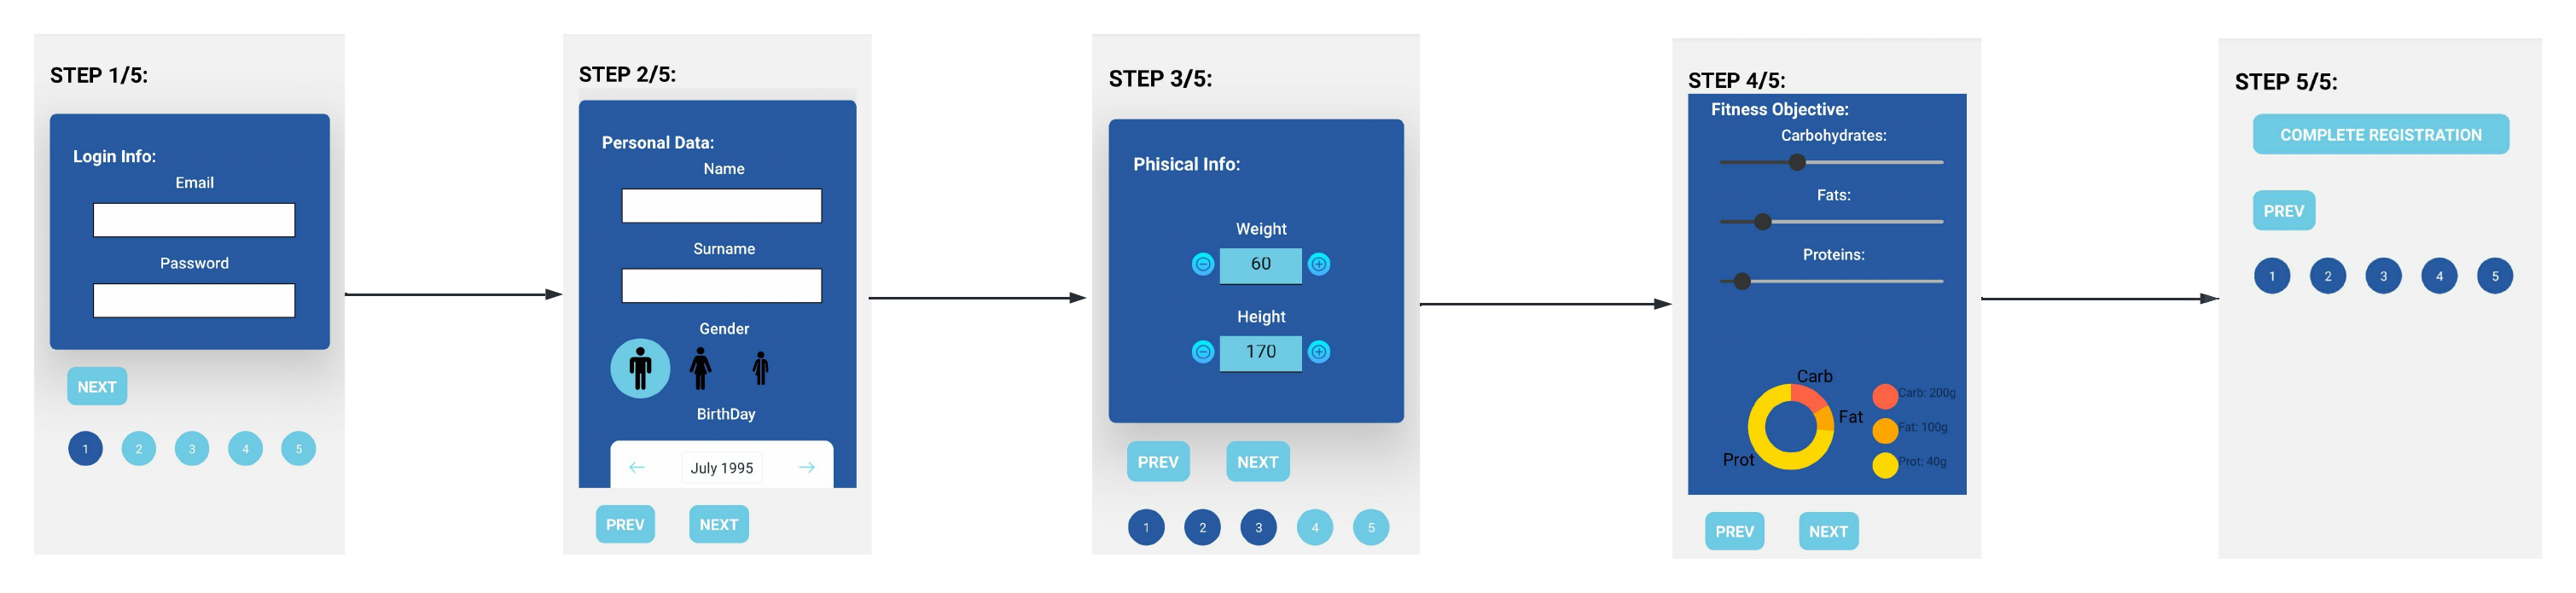
\includegraphics[scale=0.085]{Registration}
\end{center}

\paragraph{Search and Add Food}

\begin{center}
	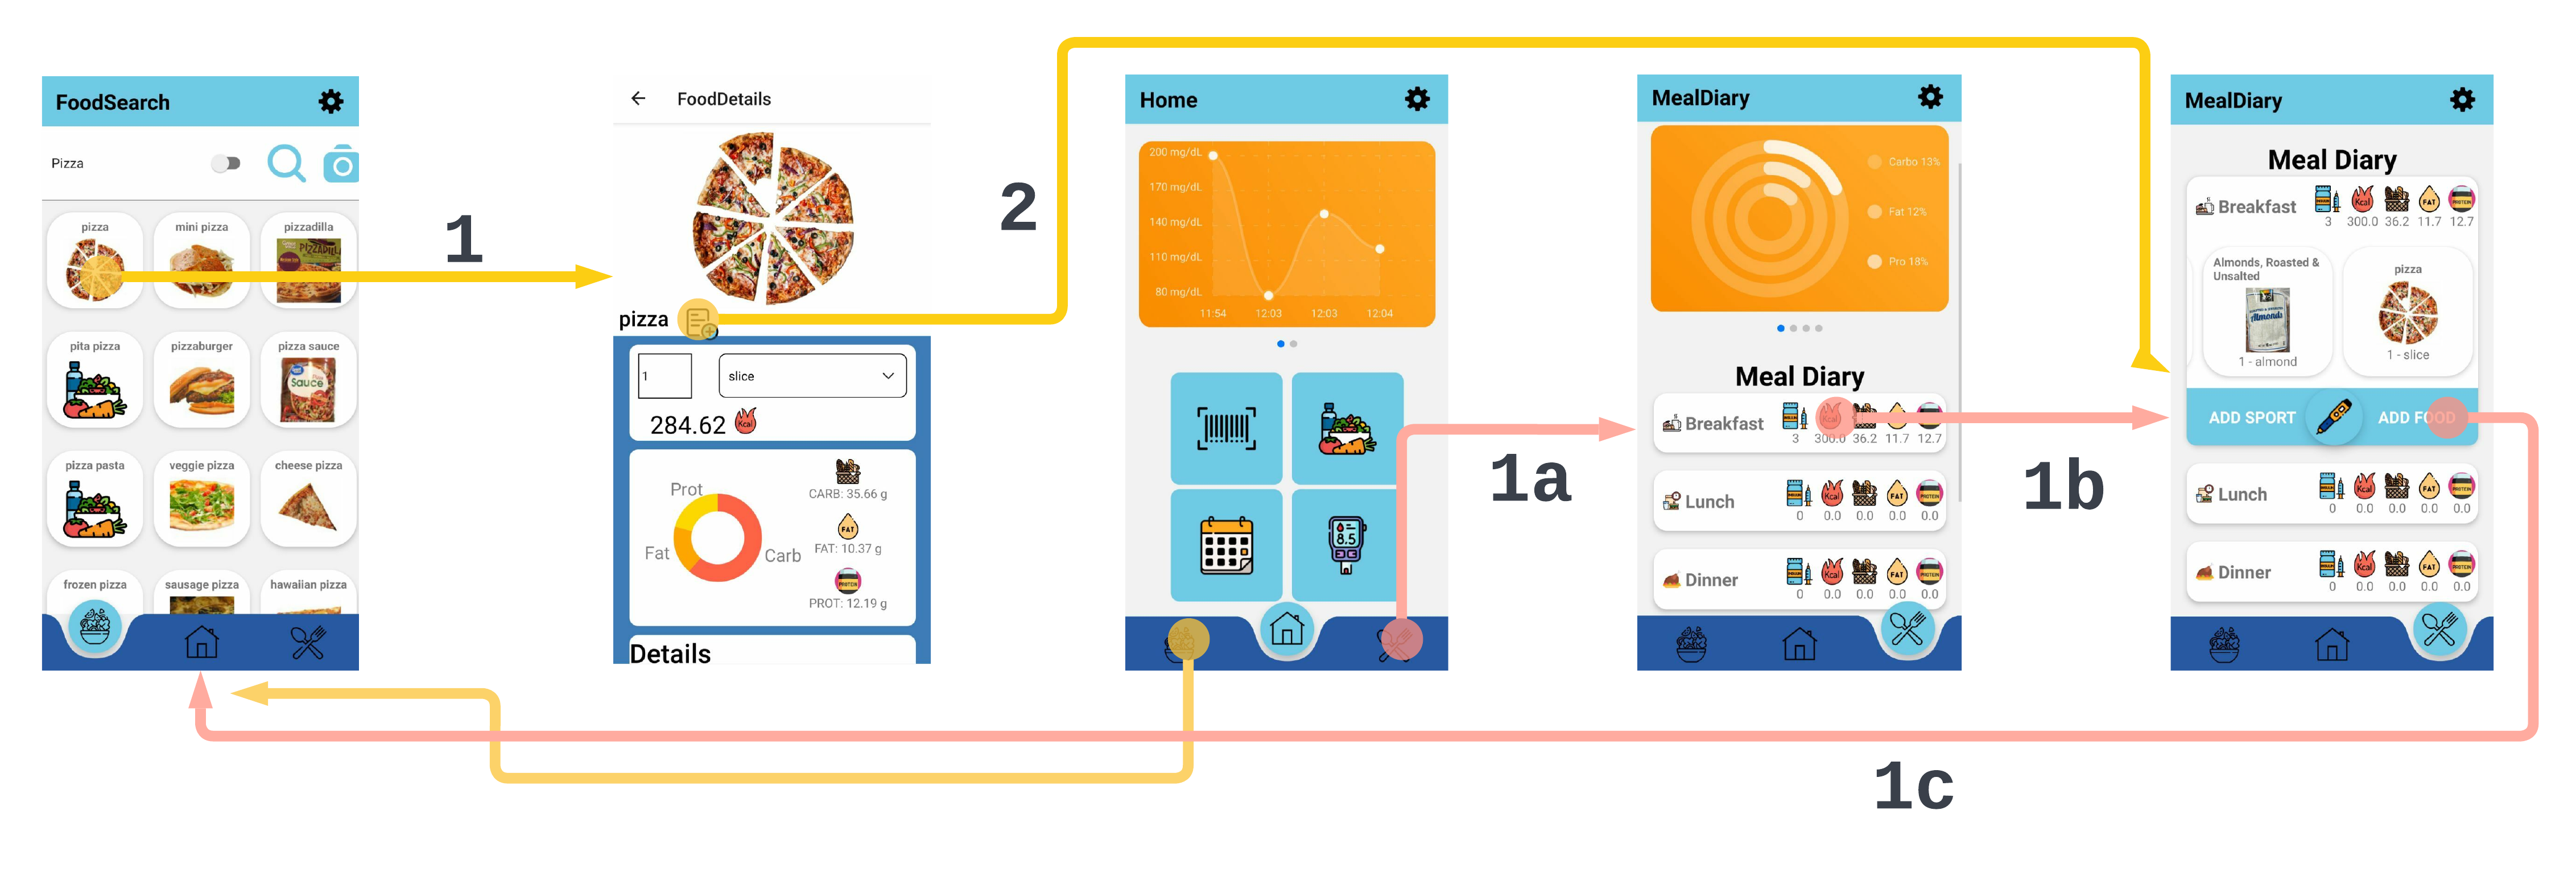
\includegraphics[scale=0.108]{Search Food}
\end{center}

\paragraph{Add Sport}
\begin{center}
	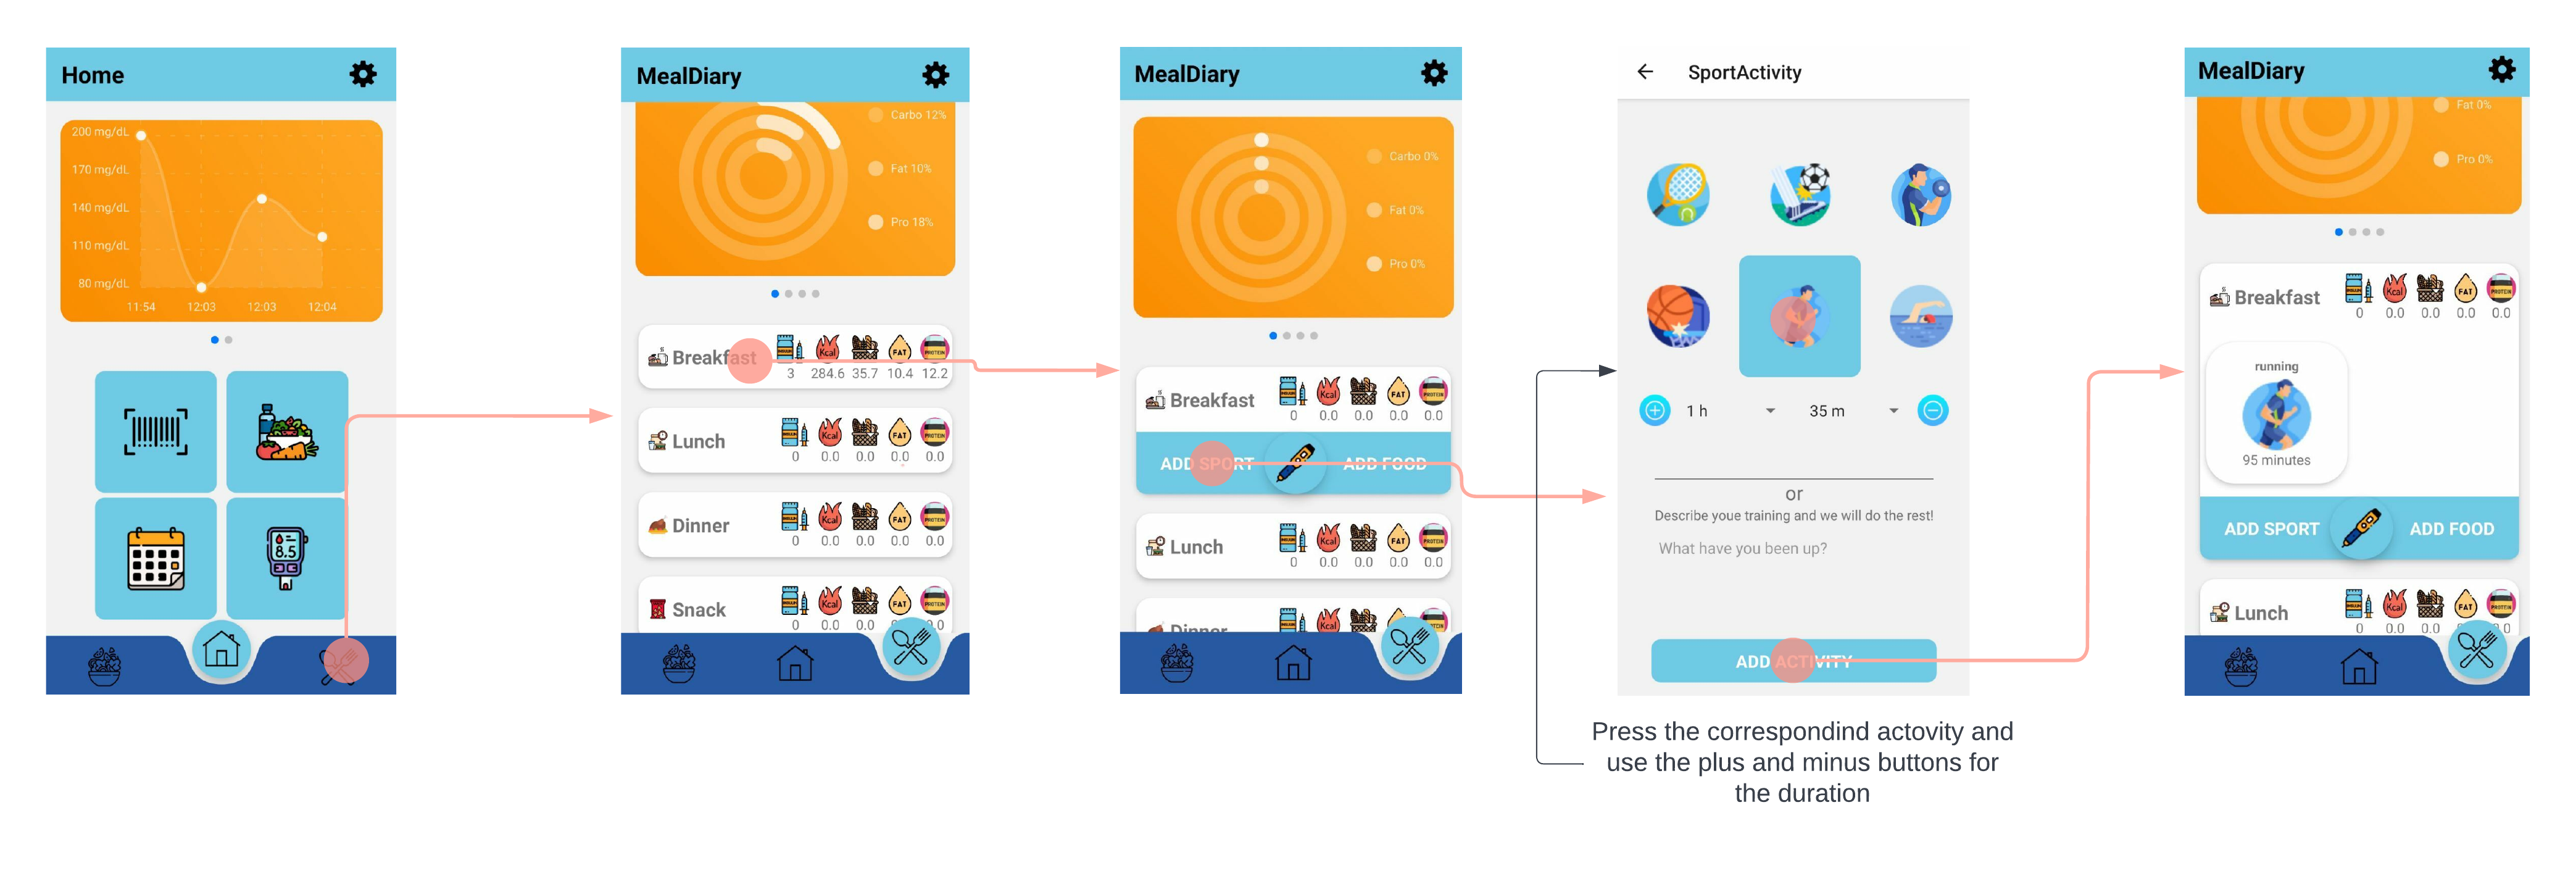
\includegraphics[scale=0.117]{Sport}
\end{center}

\newpage
\paragraph{Delete Food}

\begin{center}
	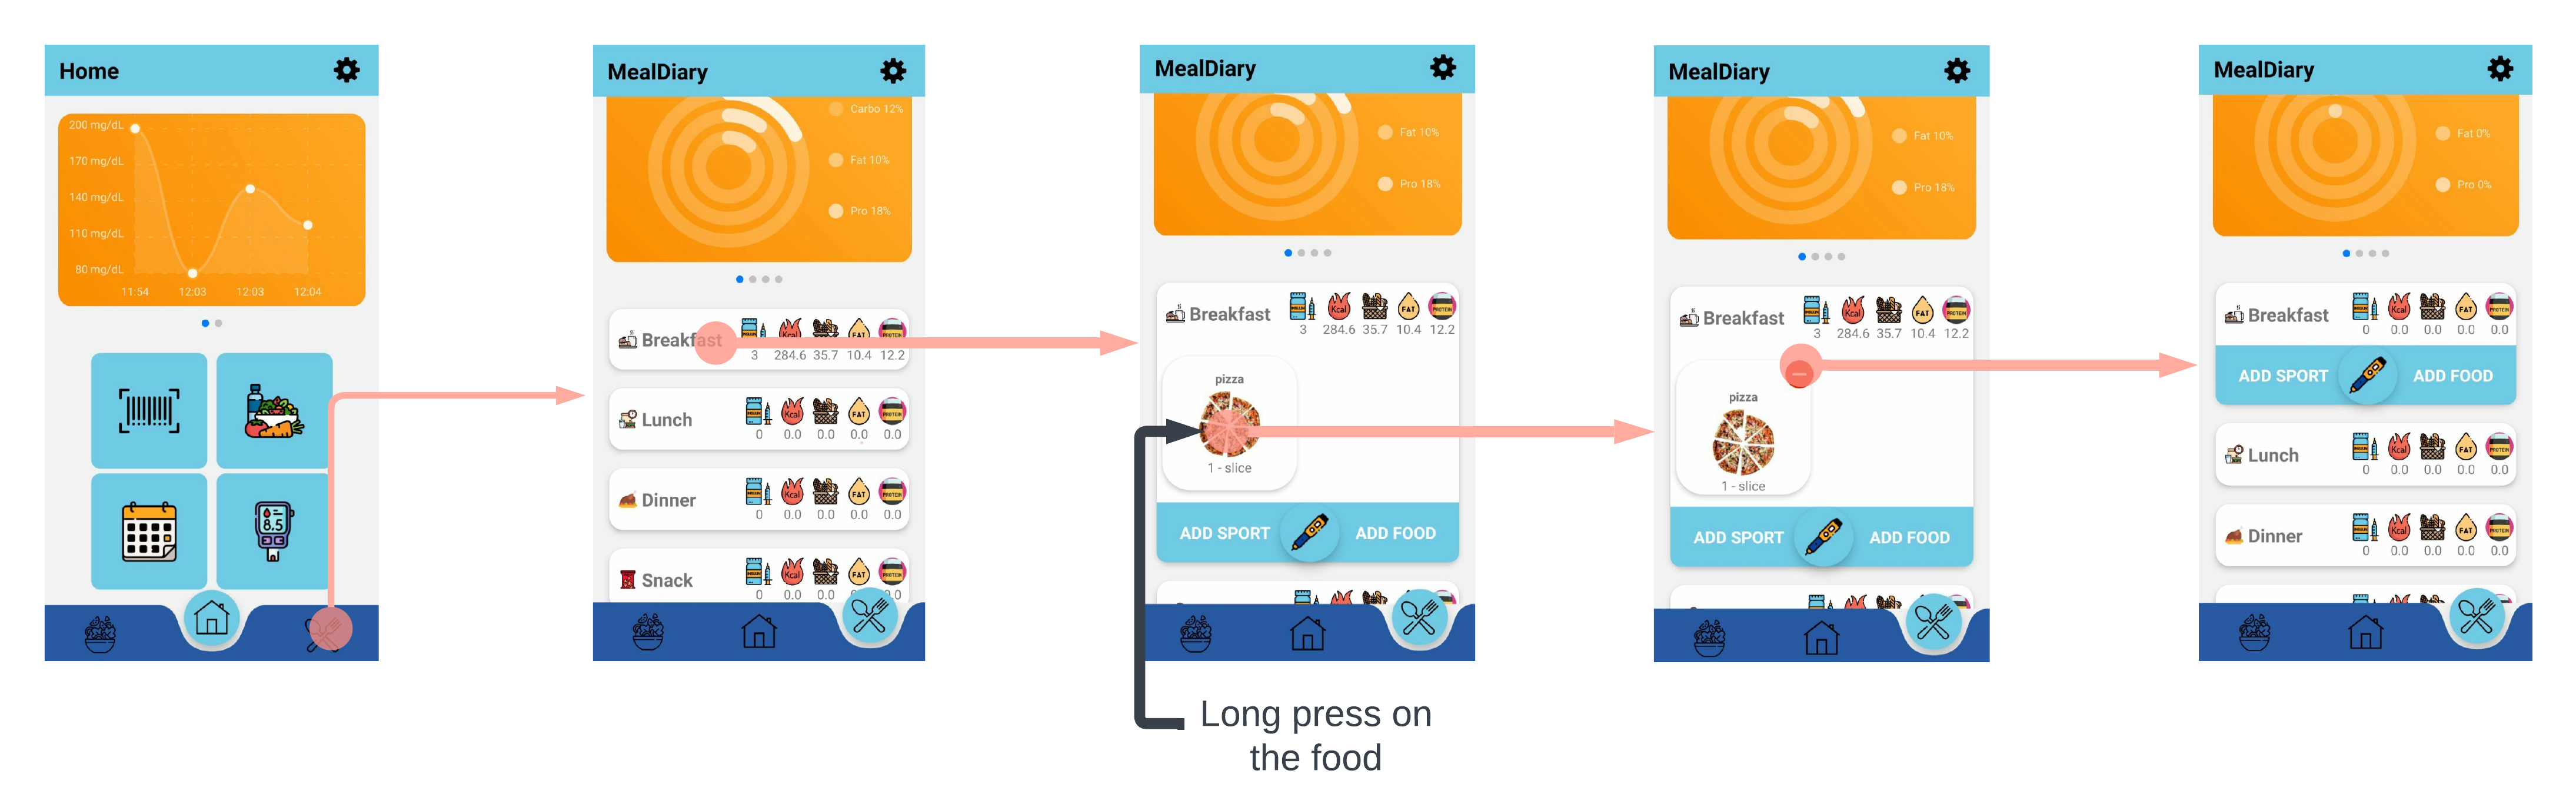
\includegraphics[scale=0.112]{Delete Food}
\end{center}


\paragraph{Calculate Insulin}
\begin{center}
	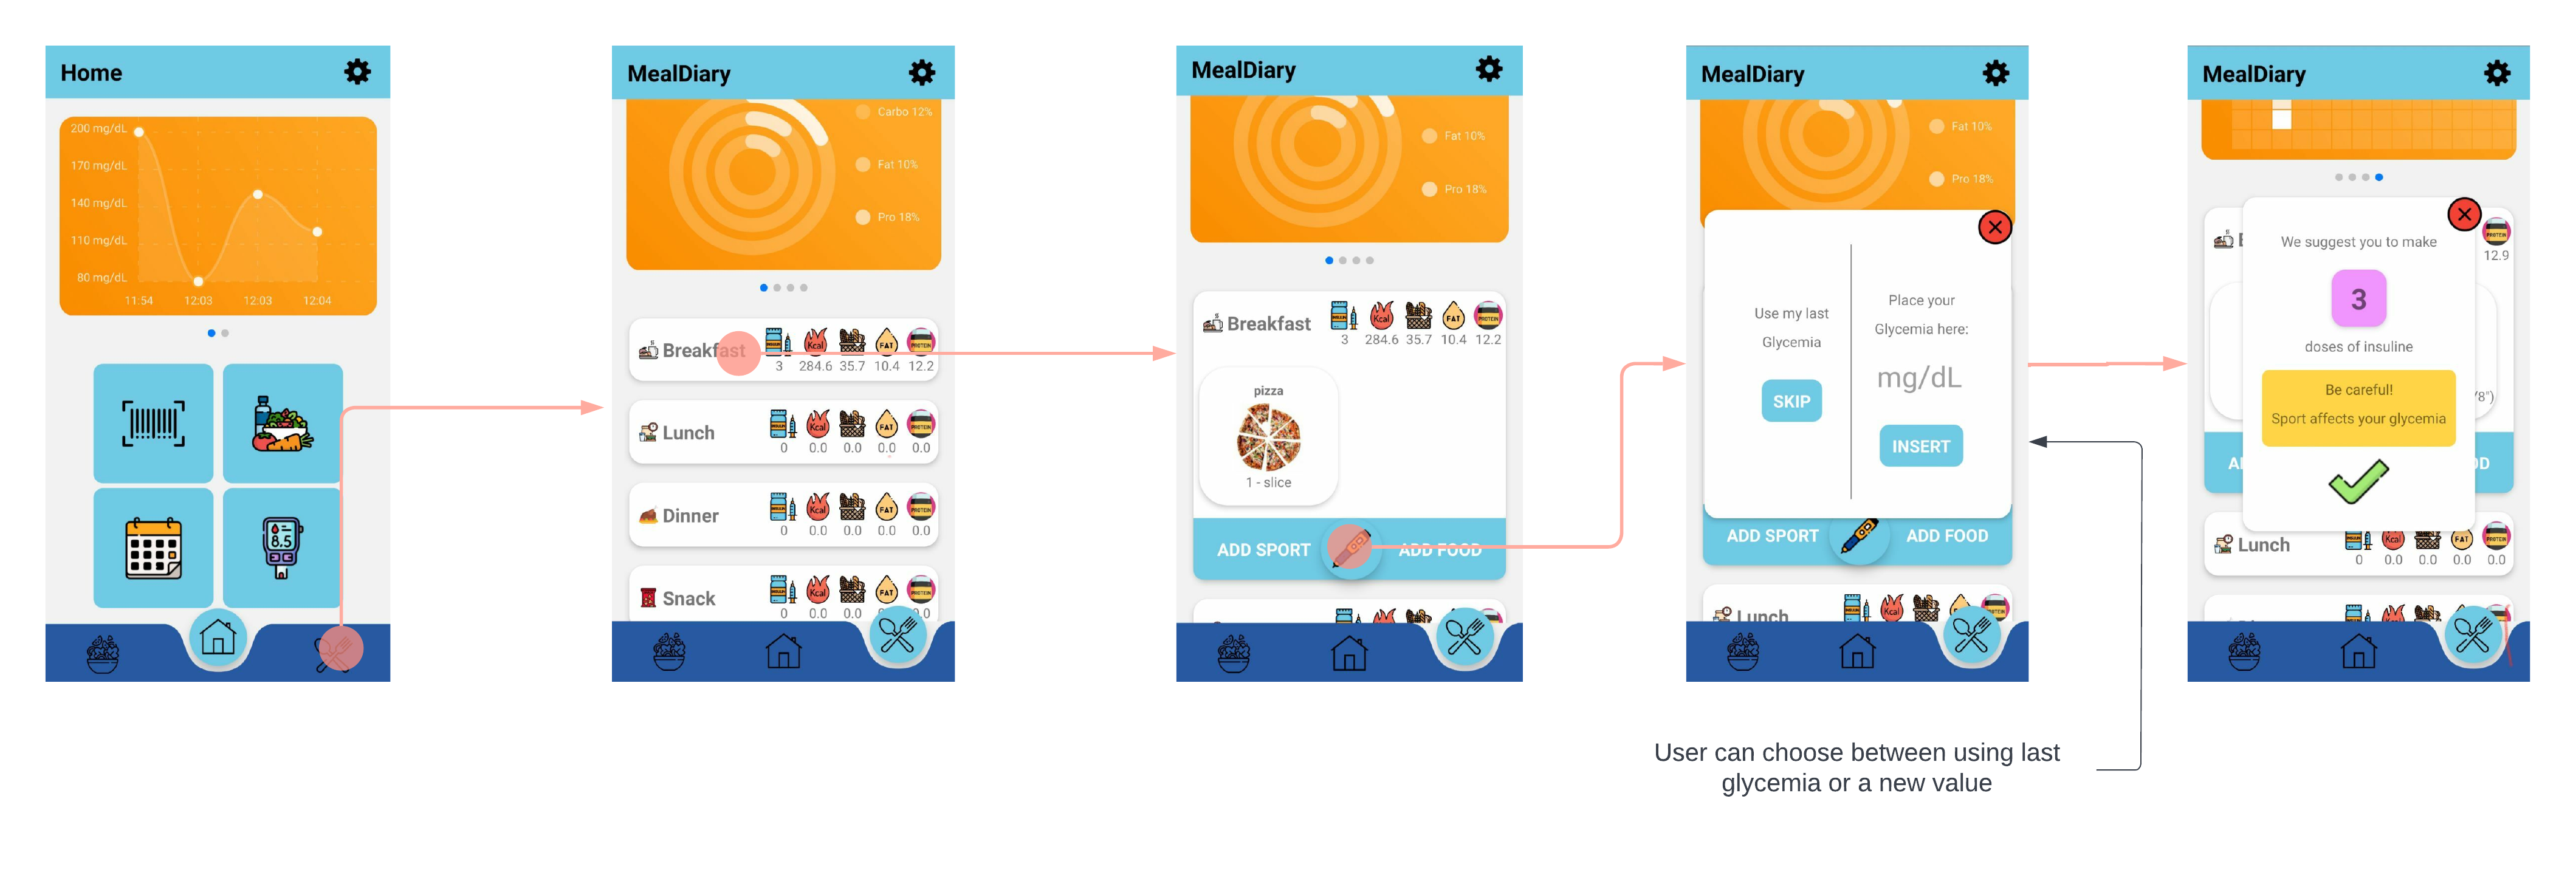
\includegraphics[scale=0.116]{Insulin Calculation}
\end{center}

\newpage
%%%%%%%%%%%%%%%%%%%%%%%%%%%%%%%%%%%%%%%%%%%%%%%%%%%%%%%%%%%
\section{Architecture}
\vspace{10.5cm}
	The technology used to make this app is react native \cite{React Native}.
	\begin{center}

	
\includegraphics[scale=0.1]{RN}
\end{center}

	\subsection{Folder Structure}
	\begin{docCommand}{assets}{}
		Contains all images and component with a proper mapping.
	\end{docCommand}

	\begin{docCommand}{constants}{}
		All constants concerning the design and states of the app.
	\end{docCommand}

	\begin{docCommand}{customComponents}{}
		All buttons, charts and pickers specifically designed for the pages.
	\end{docCommand}

	\begin{docCommand}{pages}{}
		Folder with all pages of the app, using the custom components
	\end{docCommand}

	\begin{docCommand}{stateManager}{}
		Redux States for data managing with actions and reducers: macroTracker for meals and userReducer for the patient.
	\end{docCommand}

	\begin{docCommand}{utils}{}
		Logic of API, authentication, Firebase and Insulin Calculator
	\end{docCommand}




\newpage
%%%%%%%%%%%%%%%%%%%%%%%%%%%%%%%%%%%%%%%%%%%%%%%%%%%%%%%%%%%
\section{API and Services}	
\vspace{10.5cm}	
InsuLink uses different APIs to get all informations about food and storing user data.
	\subsection{Nutritionix}\label{subsec:mathenvironments}
		Nutritionix \cite{Nutritionix} is the API used to have a well detailed food database, with all important informations 
		to have a completely working application.
		\begin{center}

			
\includegraphics[scale=0.35]{Nutritionix}
		\end{center}
		Nutritionix support Natural Language, BarCodes and has a huge dataset with food and recipes. Here there're some 
		functionalities offered by the standard plan:
		\begin{center}

			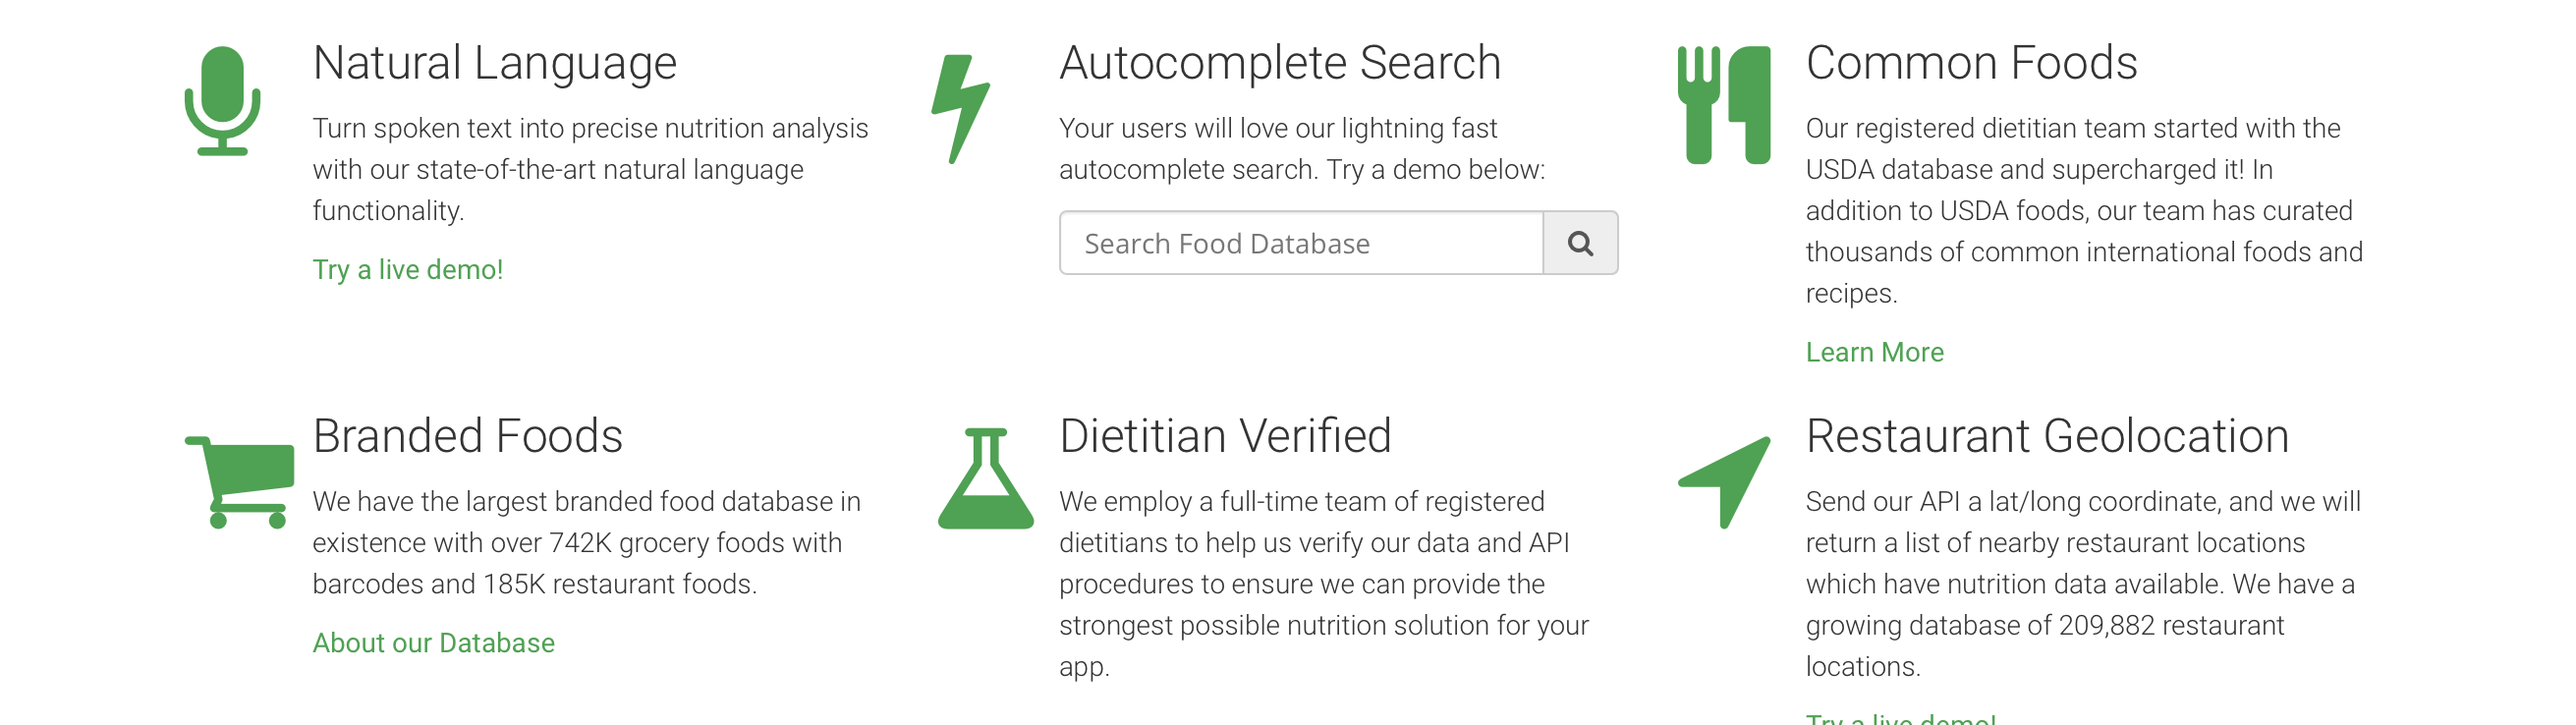
\includegraphics[scale=0.3]{Nutritionix detail}
		\end{center}
		The API requests and responses are documentend in the \textbf{\emph{/utils/apiQuery.js}} class

        \paragraph{Methods}
     Using GET requests in \textbf{doRequest} method to \emph{trackapi.nutritionix.com/v2}
		\begin{docCommand}{item}{}
			Given upc code (standard use for barcodes) returns the food packaging details.
	\end{docCommand}

	\begin{docCommand}{instant}{}
		Given a user query (Food Search page) returns a list of possible foods and recipes.
\end{docCommand}
       
       

	\subsection{Firebase}
	    Firebase \cite{Firebase} is a Google serverless platorm for application development. 
        It is a powerful tool to implement an app database and Google authentication, having many powerful tools to manage it.
		\begin{center}
			
\includegraphics[scale=0.2]{Firebase}
		\end{center}
		All its requests and responses are well documented in the \textbf{\emph{src/utils/firebaseQuery.js}} and \textbf{\emph{src/utils/auth.js}} classes.
		
\newpage
%%%%%%%%%%%%%%%%%%%%%%%%%%%%%%%%%%%%%%%%%%%%%%%%%%%%%%%%%%%
\section{Redux States}
\vspace{10.5cm}
To manage app states we opted for Redux library \cite{Redux}.
\begin{center}
	
\includegraphics[scale=0.2]{redux-logo}
\end{center}
Redux is used mostly for application state management. 
In other words, Redux maintains the state of an entire application in a single immutable state tree (object), which can't be changed directly.\\
When something changes, a new object is created (using actions and reducers).
\begin{center}
	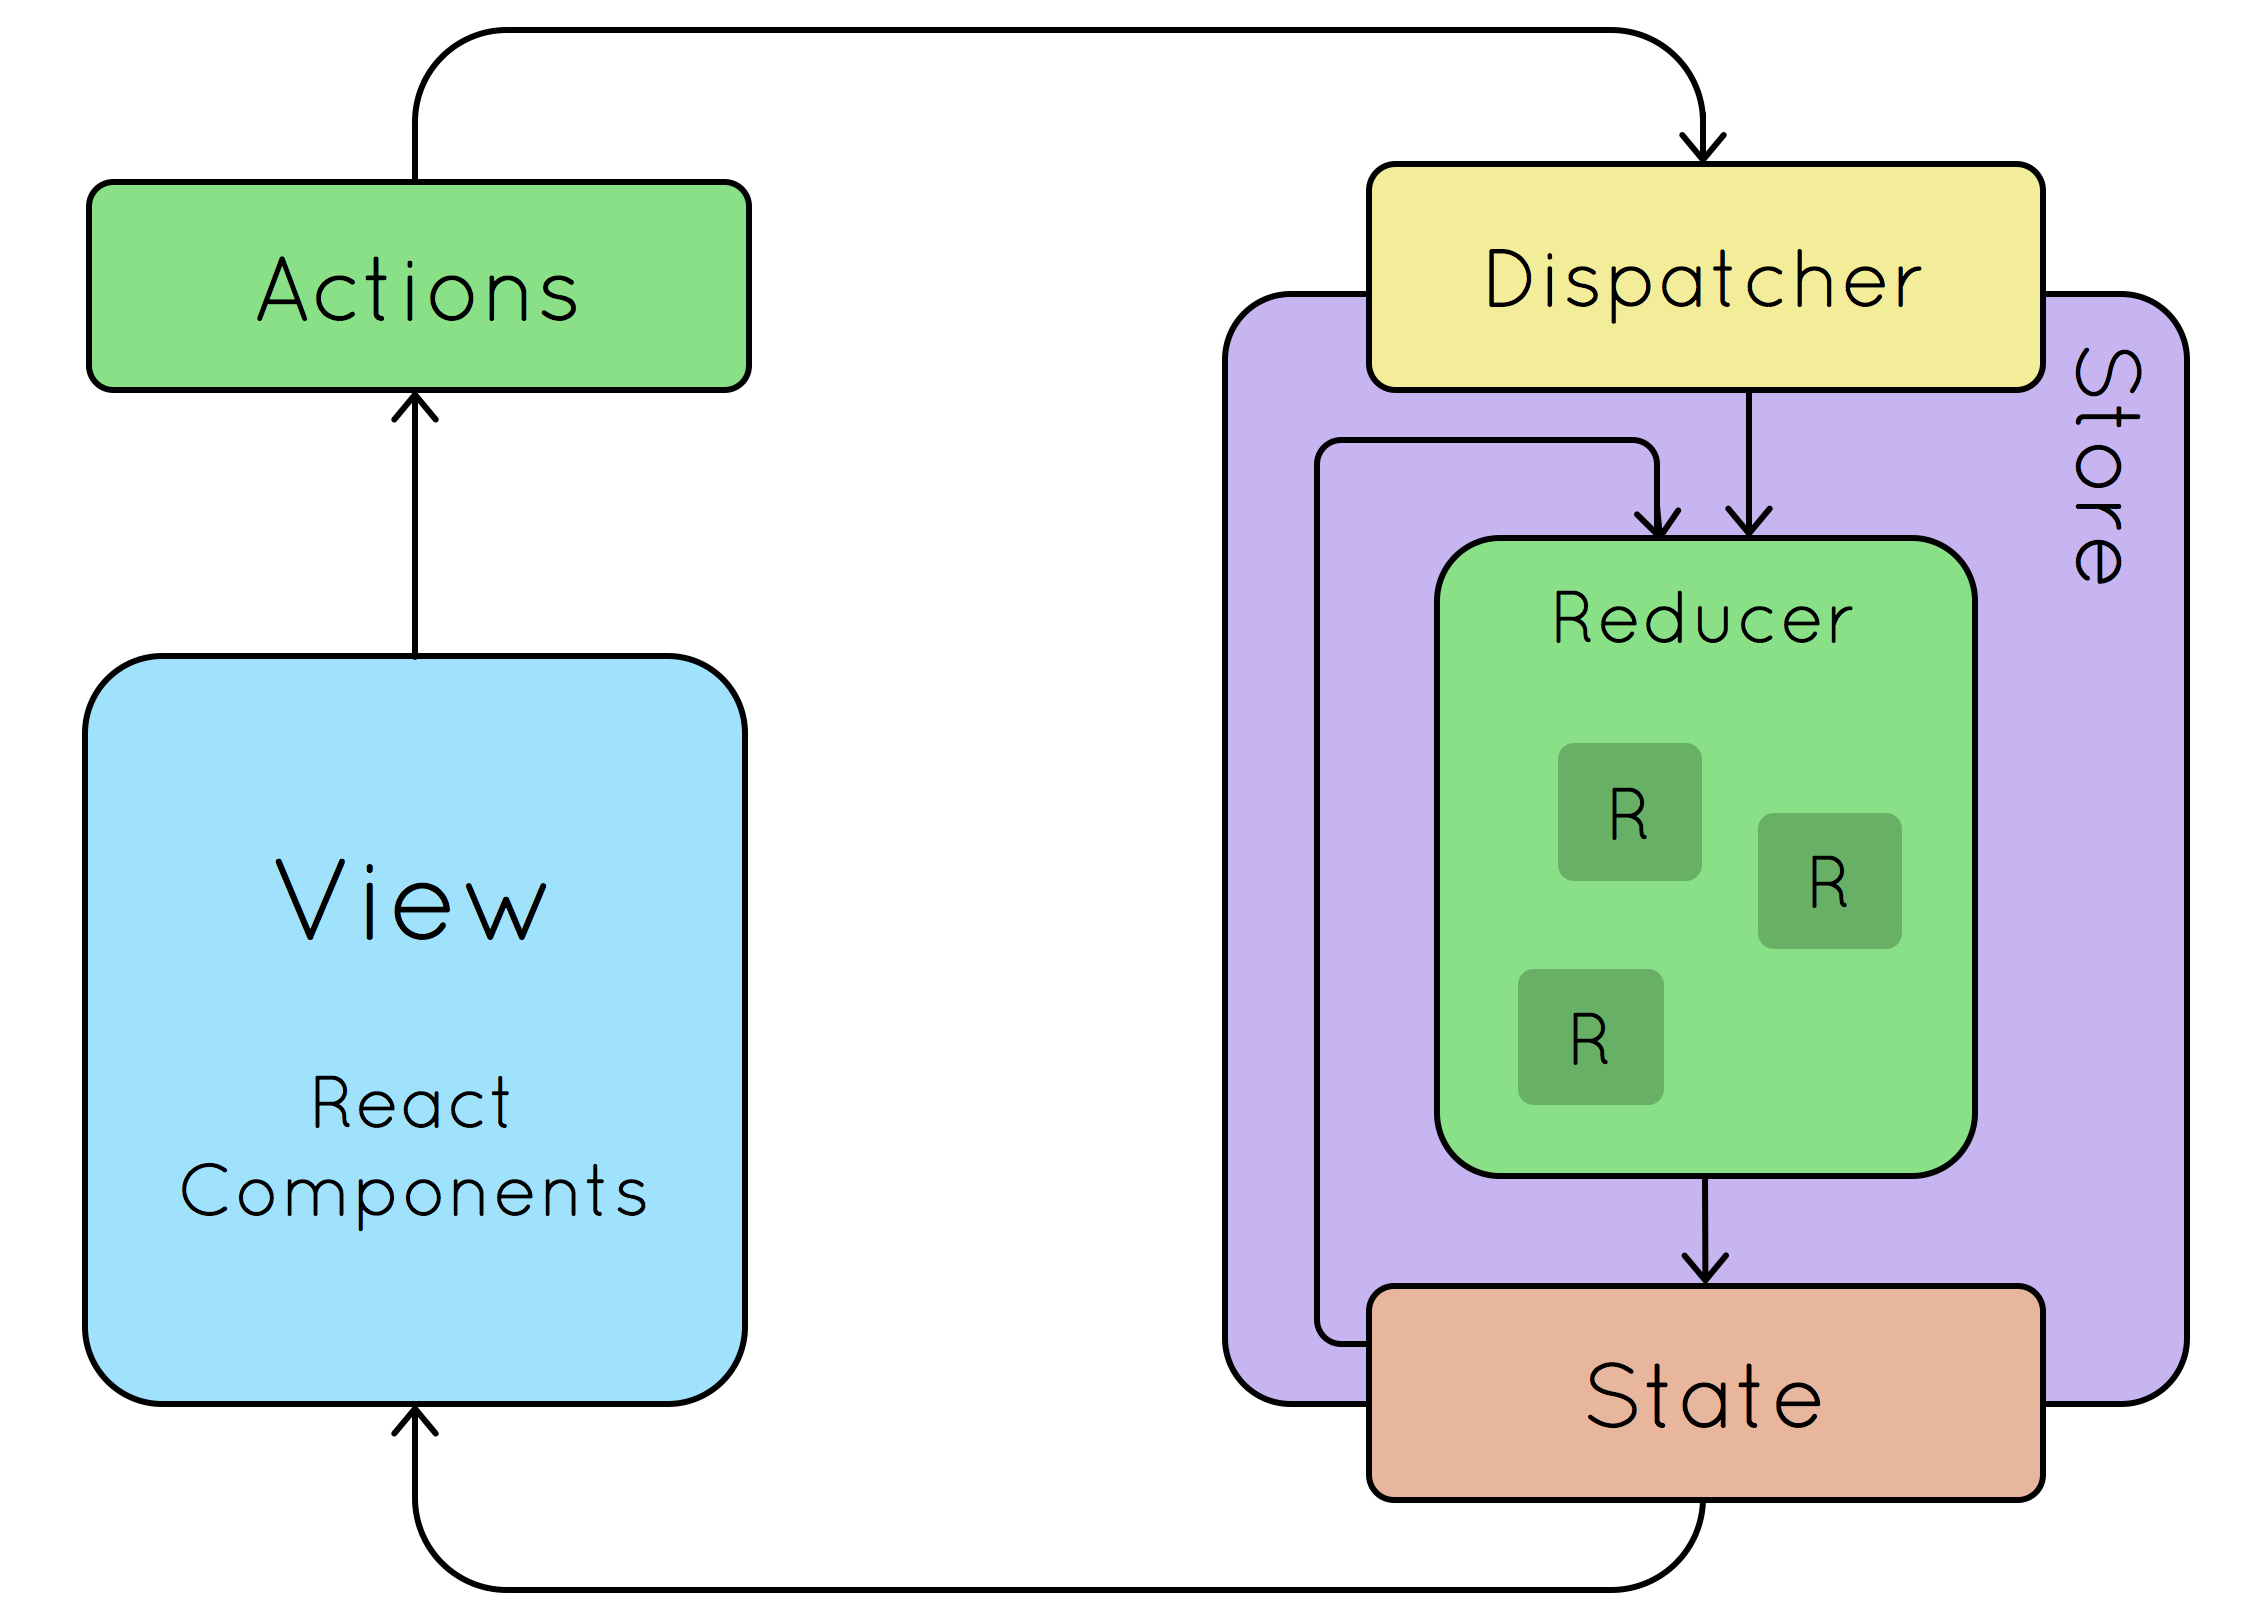
\includegraphics[scale=0.25]{Redux-workflow}
\end{center}
The main two reducers of the app are:
	\begin{docCommand}{userReducer}{}
    Contains all data about the user, including some additional fields such as
	Insulin Sensitivity Factor or CHO Ratio.\\
	If not inserted these values will be calculated considering the patient weight.

	\begin{center}
		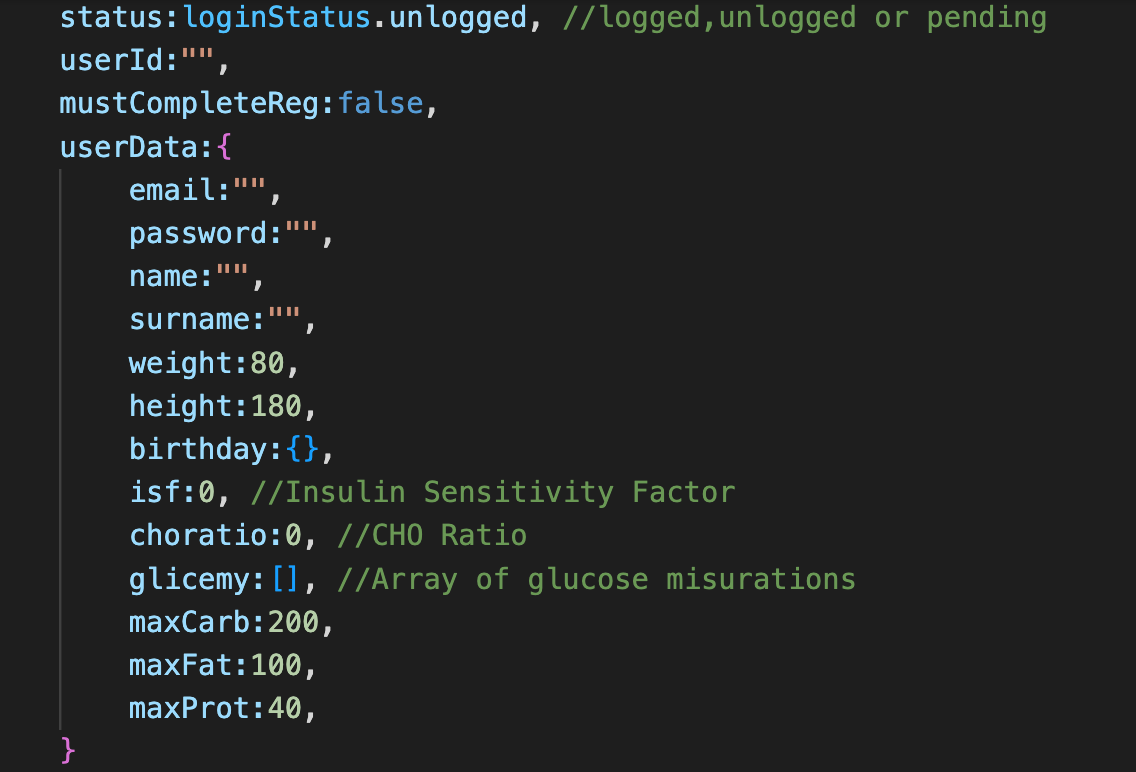
\includegraphics[scale=0.6]{userReduces}
	\end{center}

\end{docCommand}



\begin{docCommand}{macroTracker}{}
	Stores informations about each meal and sport activity of the user. Additionally, cointains 
	the sum of total macros and calories spent during the day. 
	\begin{center}
		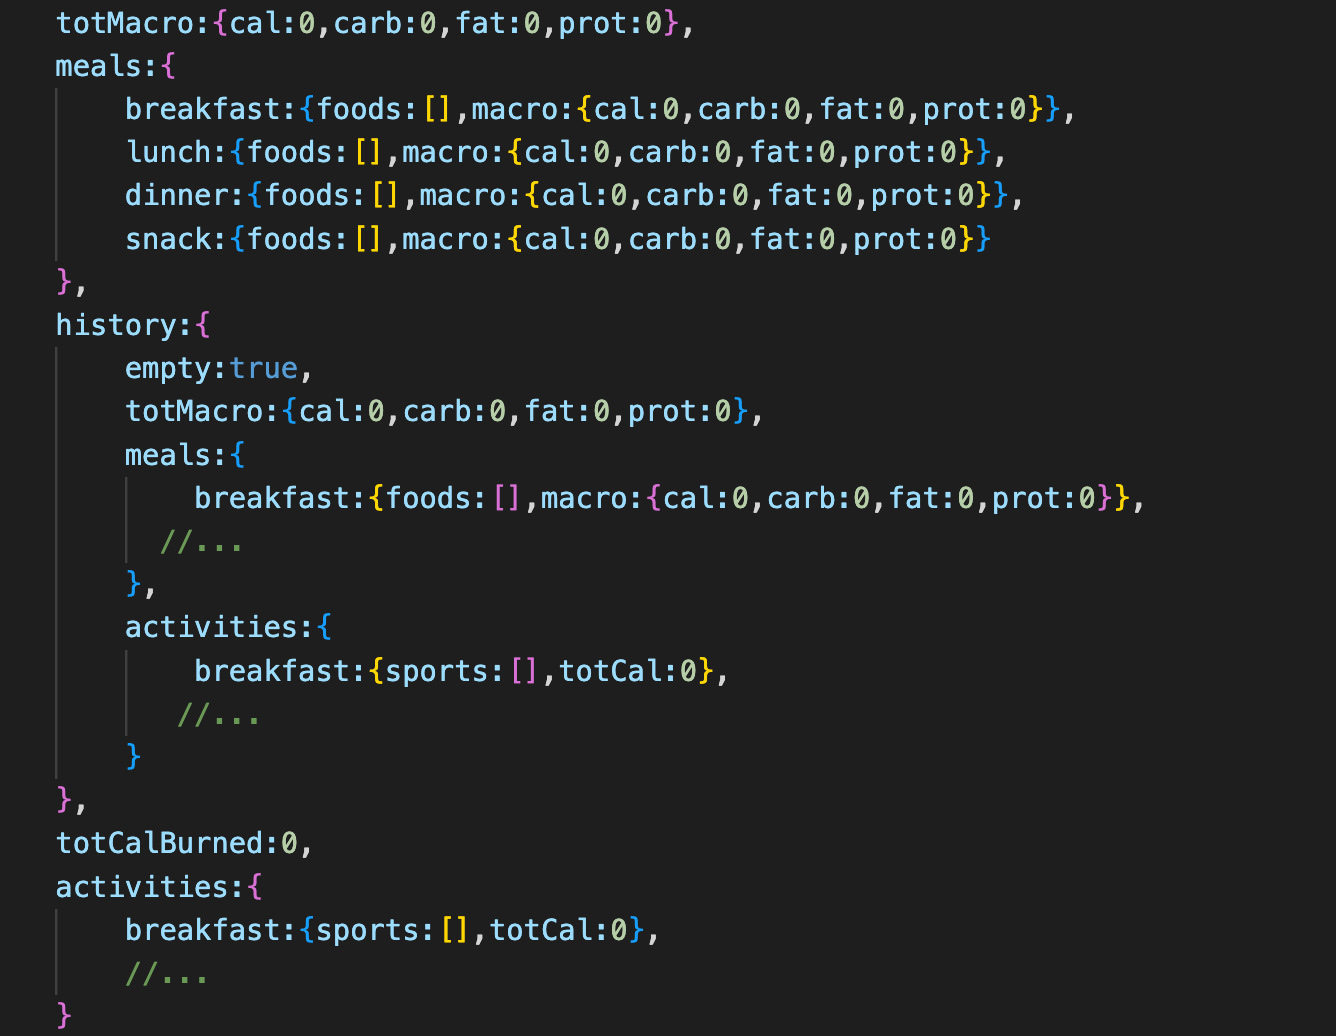
\includegraphics[scale=0.5]{macroTracker}
	\end{center}

\end{docCommand}
\newpage
\newgeometry{
		left=32mm, right=18mm, top=20mm, bottom=18mm,
		marginparwidth=28mm, marginparsep=4mm}
%%%%%%%%%%%%%%%%%%%%%%%%%%%%%%%%%%%%%%%%%%%%%%%%%%%%%%%%%%%
\section{Insulin Calculator}
\vspace{10.5cm}
To understand the algorithm behind the Insulin Calculator, here're some basics:
\begin{itemize}
 \item  Approximately 40-50 percent of the total daily insulin dose is to replace insulin overnight, when you are fasting and between meals
 \item  The other 50-60 percent of the total daily insulin dose is for carbohydrate coverage (food) and high blood sugar correction
 \item The bolus dose for food coverage is prescribed as an insulin to carbohydrate ratio. The insulin to carbohydrate ratio represents how many grams of carbohydrate are covered or disposed of by 1 unit of insulin.
 \item The bolus dose for high blood sugar correction is defined as how much one unit of rapid-acting insulin will drop the blood sugar.
 \item Sport Activity deeply influences the response to insuline and determine a less request of insulin in the patient.
\end{itemize}
Not considering sport activity, may lead the patient to a low bloodsugar value. 
Insulink checks if the user has done sport and suggests a new dose value with one unit less.
This is not true for all patients, some may need even less amount of insulin.\\
\newpage
\subsection{Formulas}
The main equation for the correct meal dose calculation is:

\begin{center} 
 CHO Insulin Dose = {$\Sigma$} grams of CHO in the meal / grams of CHO disposed by 1 unit of insulin
\end{center}

This happens in ideal conditions where glycemia is in the optimal interval.\\
Normally this is not the case: after a glucose misuration the patient could find an high
bloog sugar. In this case there's a \textbf{\emph{correction dose}}:

\begin{center} 
	High Blood Sugar Correction Dose = {$\Delta$} (Actual blood sugar - Target blood sugar) ÷ Correction Factor
\end{center}

The result formula will be:

\begin{center} 
CHO Total Dose = CHO Insulin Dose + High Blood Sugar Correction Dose
\end{center}

Moreover, there's the sport activity to take into account and it will affect the value
by decresing it. 


\newpage
\newgeometry{
	left=20mm, 
	right=20mm, 
	top=20mm, 
	bottom=20mm}
%%%%%%%%%%%%%%%%%%%%%%%%%%%%%%%%%%%%%%%%%%%%%%%%%%%%%%%%%%%
\section{Testing}
\vspace{10.5cm}

To perform automated and personalized testing it was used Jest \cite{Jest}. It is a JavaScript Testing Framework that supports React Native.
Tests were performed on:
\begin{docCommand}{__tests__}{}
Where to overcome some technological barriers, mock objects were used instead of not supported libraries.
\end{docCommand}

\subsection{Folders}


\begin{docCommand}{api-test}{}
	Local storage and API calls from Firebase and Nutritionix.
\end{docCommand}

\begin{docCommand}{redux-test}{}
	Redux and user actions such as: adding food to meal or removing it. 
\end{docCommand}

\begin{docCommand}{renders-test}{}
	Checks correct Pages rendering. Makes snapshots of all pages and compares them with expected result.
\end{docCommand}

\begin{docCommand}{utils}{}
   Checks User input and Insulin Calculator 
\end{docCommand}

At the end were performed more than 50 successful tests on the app.

\begin{center} 

\subsection{Tests}
\begin{tabular}{ |p{3cm}|p{5cm}|  }
	\hline
	\multicolumn{2}{|c|}{Nome Test} \\
	\hline
	Entry Conditions & ISO ALPHA 2 Code \\
	\hline
	Event Flows & 
	1. Open application \newline    
	2. Click on \newline    
	3. ... \newline    
	4.  
	  \\
	\hline
	Exit Conditions & AX  \\
	\hline
	Notes &AL\\
	\hline
	\end{tabular}
\end{center}


\newpage
\newgeometry{
	left=32mm, right=18mm, top=20mm, bottom=18mm,
	marginparwidth=28mm, marginparsep=4mm}
%%%%%%%%%%%%%%%%%%%%%%%%%%%%%%%%%%%%%%%%%%%%%%%%%%%%%%%%%%%
\section{Future Implementations}
\vspace{10.5cm}
Insulink has been structured with the possibility of implementing new technologies inside it.
\subsection{API}
The API utils section of the code is easly changeble from one provider to another. Using a premium API
would affect the performance but also the usability of the app.
\subsection{Machine Learning and AI}
Calculating the correct insulin dose is a really difficult problem. The factor that influences the output is not only the amount of carbohydrates eaten,
but many other features: fats, sport activity, emotional condition and sometimes even the weather.\\
Moreover each patient needs specific treatments, and has a different resistance to insulin.\\
Using Machine Learning in this field could be a smart way to correctly predict the optimal insulin dose. 

\newpage
\subsection{NFC Glucose Meter}
Some Glucose Meters use new technologies to simplify diabetic patients life. One famous example is
FreeStyle Libre \cite{FreeStyle}. Using the NFC technology to retrieve glycemia helps not only in terms 
of time but also in visualization and store of data. \\
Once implemented, the user has just to bring the phone closer to the sensor and the app will check the 
glucose (and store it).
\begin{center}

	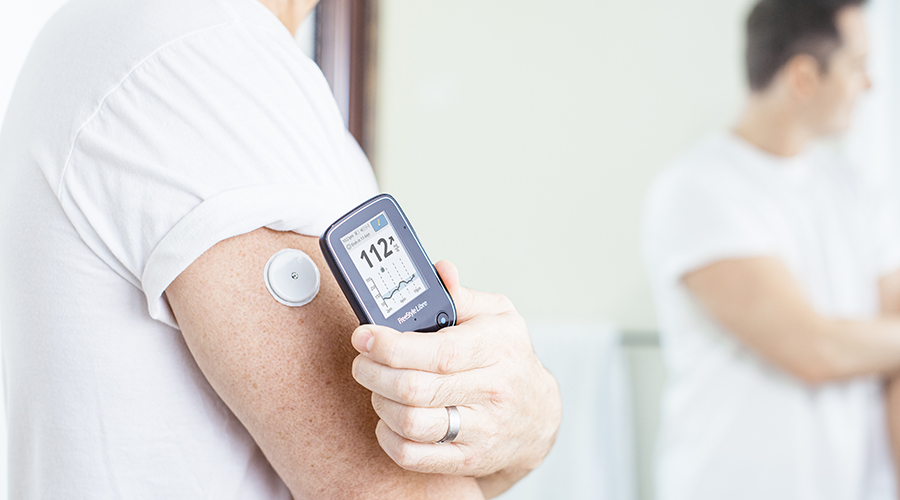
\includegraphics[scale=0.45]{FreeStyle Libre}
\end{center}


\newpage
%%%%%%%%%%%%%%%%%%%%%%%%%%%%%%%%%%%%%%%%%%%%%%%%%%%%%%%%%%%
\section{References}
\begin{thebibliography}{17}
	\vspace{10.5cm}
		\bibitem{Type 1 Diabetes} Diabetes Definition\\
				\url{https://en.wikipedia.org/wiki/Type_1_diabetes}
		\bibitem{Bolus} Bolus Definition\\
				\url{https://en.wikipedia.org/wiki/Bolus_(medicine)}
		\bibitem{React Native} React Native\\
				\url{https://reactnative.dev}
		\bibitem{Nutritionix} Nutritionix\\
				\url{https://www.nutritionix.com}
		\bibitem{Jest} Jest\\
				\url{https://jestjs.io}
		\bibitem{Firebase} Firebase\\
				\url{https://firebase.google.com}
		\bibitem{FreeStyle} FreeStyle Libre\\
				\url{https://www.freestyle.abbott/us-en/home.html}
		\bibitem{Redux} Redux\\
				\url{https://redux.js.org}	
		\bibitem{Insulin Dose} Source for Insulin Calculator\\
				\url{https://dtc.ucsf.edu/types-of-diabetes/type1/treatment-of-type-1-diabetes/medications-and-therapies/type-1-insulin-therapy/calculating-insulin-dose/}
	\end{thebibliography}
\addtocounter{section}{14}
\addcontentsline{toc}{section}{\protect\numberline{\thesection}~~~ References}
%%%%%%%%%%%%%%%%%%%%%%%%%%%%%%%%%%%%%%%%%%%%%%%%%%%%%%%%%%%%%%%%%%
\end{document}